A vista superior da estrutura do pórtico pode ser visualizada na representação abaixo:

\begin{figure}[H]
  \centering
  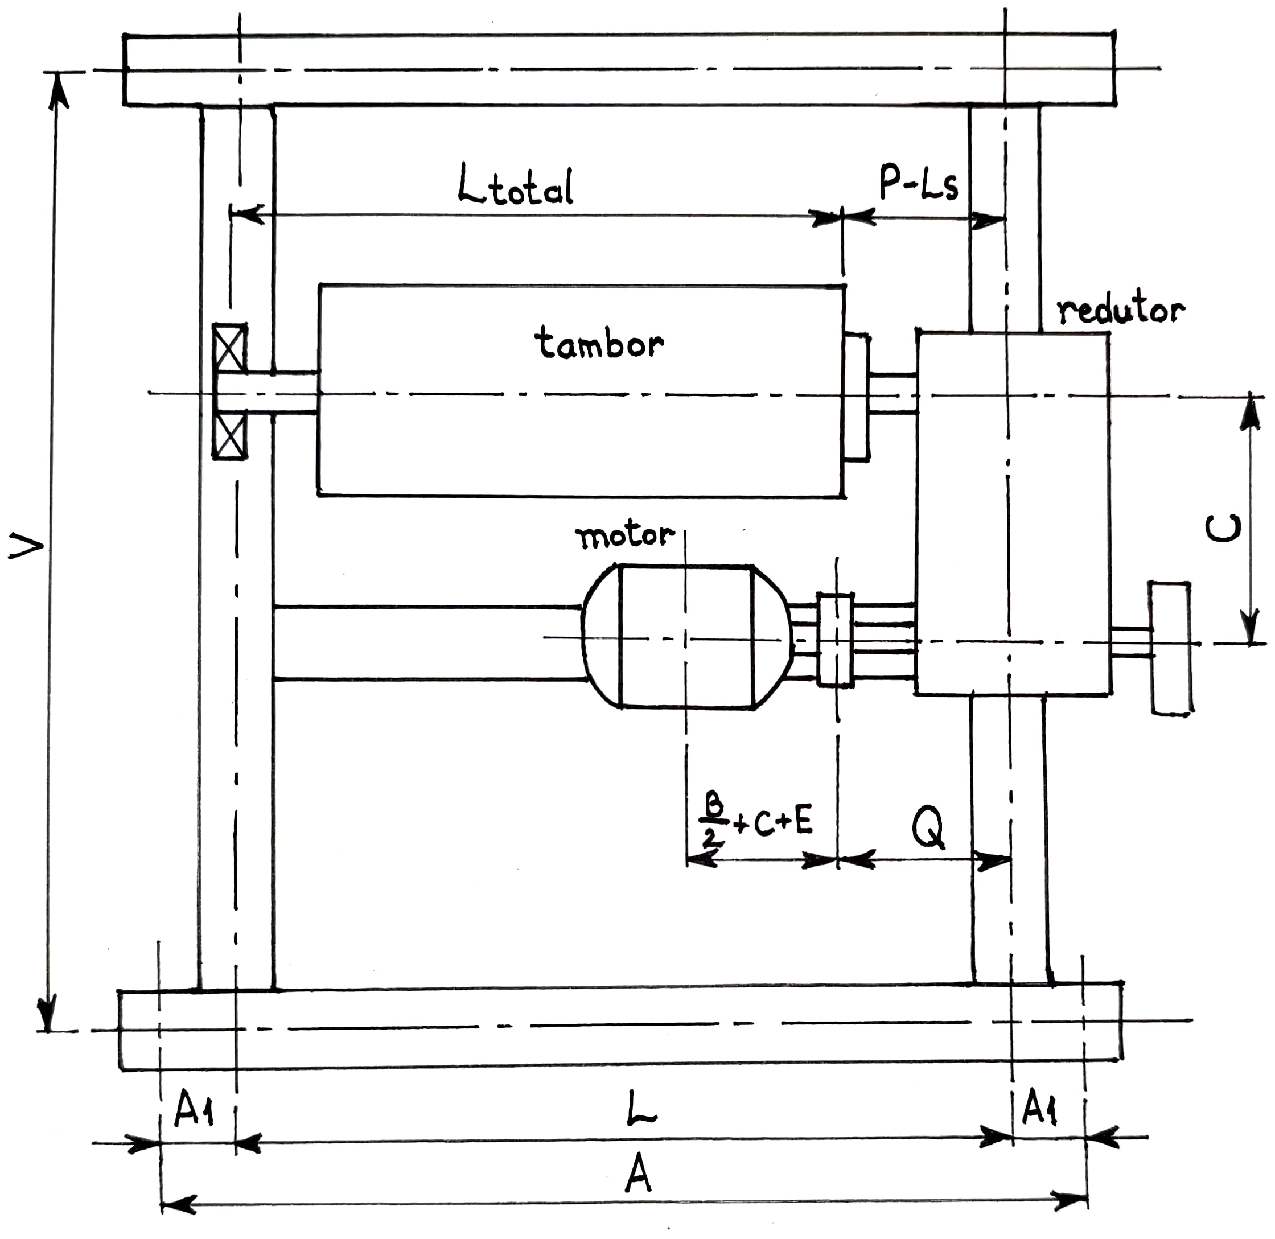
\includegraphics[width=0.9\textwidth]{content/sections/04_estrutura/figures/estrutura.pdf}
  \caption{Vista superior da estrutura do pórtico (Autor)}
  \label{fig:estrutura}
\end{figure}

As cargas atuantes na estrutura, considerando o peso dos componentes, são as seguintes:

\begin{figure}[H]
  \centering
  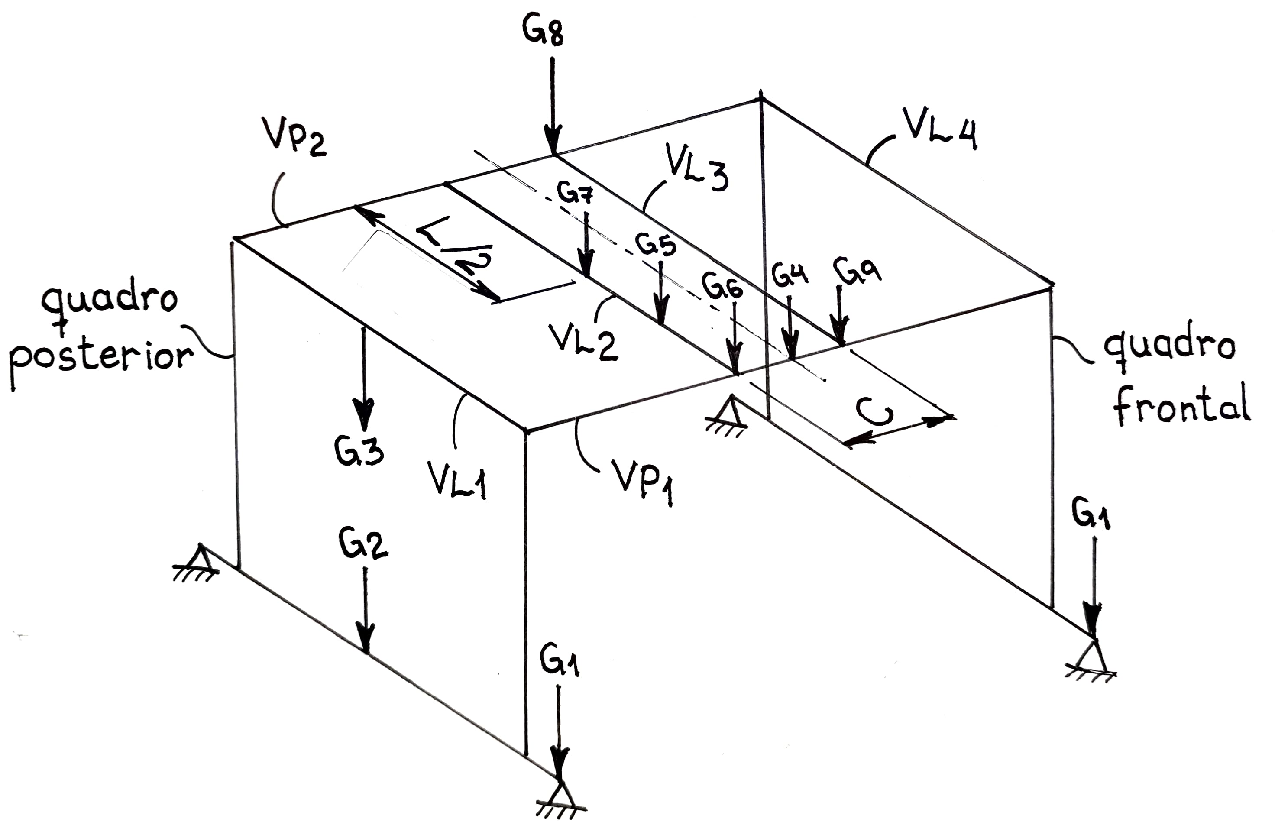
\includegraphics[width=0.9\textwidth]{content/sections/04_estrutura/figures/cargas_estrutura.pdf}
  \caption{Cargas atuantes na estrutura do pórtico (Autor)}
  \label{fig:cargas_estrutura}
\end{figure}

O material utilizado nas vigas é o aço estrutural ASTM A36.
